%!TEX program = xelatex
%!TEX TS-program = xelatex
%!TEX encoding = UTF-8 Unicode

\chapter{从Google 说起}

\section{Google}
英语中哪个字母最重要?很多人都会回答说是字母 $e$,因为字母 $e$ 的使用频率最高。下表列出了26个英语字母的使用频率。那么数学中哪个字母最重要呢?这个问题可能会变得很有争议,但是字母 $e$ 绝对是一个相当有竞争力的候选。接下来就讲讲和字母 $e$ 相关的数学故事。

\begin{table}[htbp]
\centering
\begin{tabular}{|l|}
\hline
A 8.19 B 1.47 C 3.83 D 3.91 E 12.25      \\ \hline
F 2.26 G 1.71 H 4.57 I 7.10 J 0.14       \\ \hline
K 0.41 L 3.77 M 3.34 N 7.06 O 7.26       \\ \hline
P 2.89 Q 0.09 R 6.85 S 6.36 T 9.41       \\ \hline
U 2.58 V 1.09 W 1.59 X 0.21Y 1.58 Z 0.08 \\ \hline
\end{tabular}
\caption{英文字母使用频率}
\centering
\end{table}

故事从一个互联网公司 Google 说起。Google 是一个大家都很熟悉的公司,她造就了世界上最庞大的搜索引擎之一,而且提供了大量的互联网产品和服务,以免费的形式提供给全世界的用户使用。如果把互联网比作江湖,那么Google、Amazon、Facebook、Yahoo 这些公司都是来自美国的江湖大侠。同样地 BAT--百度、阿里和腾讯这三家公司是来自中国的大侠。那谁会是这个互联网江湖的武林盟主呢?绝大多数人会推举 Google 作为互联网江湖的武林盟主。天下武功出少林,互联网的大多数技术都源自 Google。Google 成为了计算机工程师(俗称码农)朝圣的地方,很多计算机系的毕业生在毕业时都希望能进入 Google,只要在 Google 学了一招半式,脑门上就会有技术的光环,出来以后在互联网江湖里就会变得非常值钱,受人尊重。

\section{Google 名字的由来}
Google 是一家非常具有数学基因的大公司,她是一个数学的超级大粉丝。很多活动和事件中都反映出 Google 对数学的热爱。Google 本身是一个数学名词,她表示1后面跟着100个零(即10的100次方)。这个词汇由美国数学家Edward Kasner 的外甥 Milton Sirotta 创造,之后随着 Kasner 和 james Newman 合著的《数学和想象》(Mathematics and the Imagination) 一书而广为流传。Google 的创始人套用此术语,体现了公司整合网上海量信息的远大目标。

\section{Google 数学涂鸦}
第二个反映 Google 数学基因的例子就是 Google Doodle,Google 会在一些重要的日子把 Logo 换成经过专门设计的图形,用来纪念跟这个重要日子相关的人物或事件。Google 的数学涂鸦很多很多,下面就列举一些比较有名的涂鸦。

\begin{figure}[htbp]
\centering
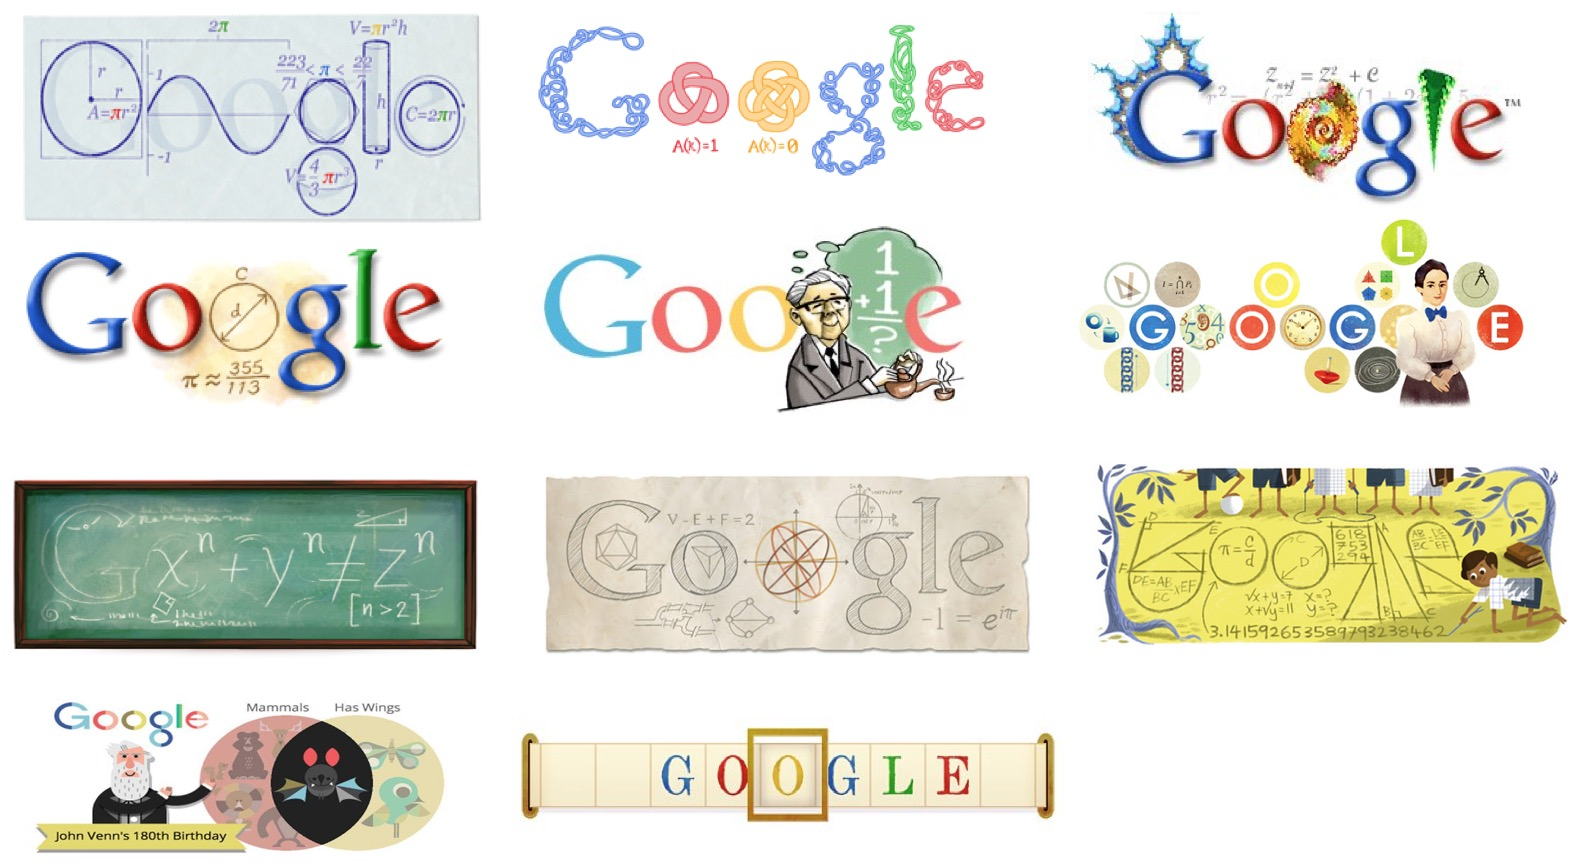
\includegraphics[scale=0.2]{google/doodle.png}
\caption{Google 数学涂鸦}
\centering
\end{figure}

从左到右,从上到下分别是2014年3月14日\href{http://www.google.com/doodles/pi-day?hl=zh-CN}{圆周率日},2010年10月11日\href{http://www.google.com/doodles/cahit-arfs-100th-birthday?hl=zh-CN}{贾希特·阿尔夫诞辰100周年},2004年2月2日\href{http://www.google.com/doodles/gaston-julias-111th-birthday?hl=zh-CN}{加斯顿·朱丽亚诞辰111周年},2009年4月20日\href{http://www.google.com/doodles/zu-chongzhis-birthday?hl=zh-CN}{祖冲之诞辰纪念日},2011年11月12日\href{http://www.google.com/doodles/hua-luogengs-101st-birthday?hl=zh-CN}{华罗庚诞辰101周年},2015年3月23日\href{http://www.google.com/doodles/emmy-noethers-133rd-birthday?hl=zh-CN}{埃米·诺特诞辰 133 周年},2011年8月17日\href{http://www.google.com/doodles/pierre-de-fermats-410th-birthday?hl=zh-CN}{皮埃尔·德·费玛诞辰410周年},2013年4月15日\href{http://www.google.com/doodles/leonhard-eulers-306th-birthday?hl=zh-CN}{莱昂哈德·欧拉诞辰306周年},2012年12月22日\href{http://www.google.com/doodles/srinivasa-ramanujans-125th-birthday?hl=zh-CN}{斯里尼瓦瑟·拉马努金诞辰125周年},2014年8月4日\href{http://www.google.com/doodles/john-venns-180th-birthday?hl=zh-CN}{约翰·维恩诞辰180周年},2012年6月23日\href{http://www.google.com/doodles/alan-turings-100th-birthday?hl=zh-CN}{阿兰·图灵诞辰100周年}。

\section{Google IPO 金额}
Google 2014年8月19日在纳斯达克 IPO, 提交的 IPO S-1 表格上写的金额是2,718,281,828美元,这个数字一给出,华尔街一片哗然,不知道 Google 为什么选择这样一个奇怪的数字,而且有零有整,精确到一美元,直接宣布融资27.1亿美元不就行了。一般公司上市的时候会选择的融资额会精确到千万、百万美元等,几乎没有精确到一美元的。但是数学的粉丝一看到这个数字,非常的兴奋,他们对这个数字再熟悉不过了。这个数就是无理数 $e$ 的前十位。上市对一个公司来说可以算最重要的事件,Google 选择在上市的时候选择这样一个融资额度,充分表达了 Google 对 $e$ 的喜爱和致敬。

\section{Google 办公楼命名}
大家都知道,数学中有三个非常著名的无理数, 圆周率 $\pi$、自然常数 $e$ 和 黄金分割比 $\phi$ , Google 对这三大无理数都特别喜欢。Google 第二幢办公楼的名称就叫 $e$,第三幢办公楼叫 $\pi$,第四幢楼则命名为 $\phi$。
\begin{figure}[htbp]
\centering
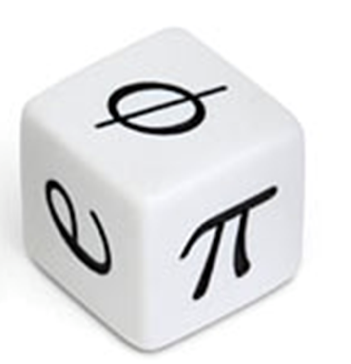
\includegraphics[scale=0.5]{google/dice.png}
\caption{三大无理数}
\centering
\end{figure}

\section{Google 招聘广告}
Google 对数学的喜爱无处不在。2004年7月在美国加州硅谷101公路的旁边出现了一个大大的广告牌,广告牌特别奇怪,只有一行字,"$\{$the first 10-digit prime in consecutive digits of $e$ $\}$.com",如图三所示。很快,类似的广告牌纷纷出现在了西雅图、哥伦比亚、马塞诸塞、华盛顿、奥斯丁、德克萨斯等美国各大州,引起了极大的关注度。很多人不禁感到奇怪,哪个公司这么有钱,打这么一个谁也看不懂的奇怪广告。数学粉丝们一看就知道这是一个数学题,常数 $e$ 中出现的第一个10位质数,很多数学粉丝纷纷开始了挑战。数学爱好者们写完程序,算出来这个数字是7427466391,然后登录 7427466391.com,发现网站里面又出现了一道新的数学题,比广告牌里的数学题还难。数学爱好者们又被这道题所吸引,攻克完这道题之后,接下来又遇到了几道题,经过层层攻克之后,数学爱好者们最终看到了 Google Lab 的一个招聘页面,大家终于明白原来那个奇怪的广告牌是 Google 公司的一个招聘广告。Google 的工程师们选择了 $e$ 这样一个无理数作为面试题,也充分表达了对无理数 $e$ 的喜爱。
\begin{figure}[htbp]
\centering
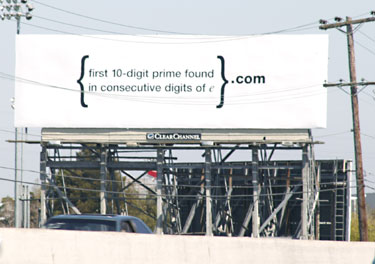
\includegraphics[scale=0.8]{google/billboard.jpg}
\caption{Google 招聘广告}
\centering
\end{figure}
	
\section{$e$ 是什么}
讲完了 Google 和 $e$ 的故事,最后来看看 $e$ 到底是什么?中学里我们就接触过 $e$,那时候我们知道 $e$ 约等于 2.718281828,$e$ 是自然对数的底数,$e$ 的定义是一个极限。
\begin{equation}
\nonumber
\begin{split}
e \approx 2.718281828 \\
ln(x) = log_{e}(x) \\
e = \lim_{n \to \infty}(1+\frac{1}{n})^n
\end{split}
\end{equation}
在上大学学习微积分、概率论、数学分析以后就会接触到越来越多跟 $e$ 相关的知识。$e$ 到底是一个什么样的数? $e$ 有什么有趣的性质?$e$ 和我们的日常生活有什么联系?历史上数学家是如何发现 $e$ 的?$e$ 有多少年的历史? 为何以 $e$ 为底的对数称为自然对数? 为什么 $e$ 有那么多名字?自然常数、欧拉常数、纳皮尔常数。为什么 Google 和许多数学人如此喜欢 $e$?
最后放上一张由字母 $e$ 组成的单词图片,这个图片里面的每一个单词背后都跟 $e$ 的某些性质相关。著名的数学科普大师马丁·加德纳(Martin Gardner,1914年10月21日—2010年05月22日)发现,三个无理数——圆周率 $\pi$、自然常数 $e$ 和 黄金分割比 $\phi$——中,学生们对自然常数 $e$ 是最不熟悉的,如果读者也不熟悉的话,欢迎接下来的时间一起学习关于 $e$ 的传奇故事。
\begin{figure}[htbp]
\centering
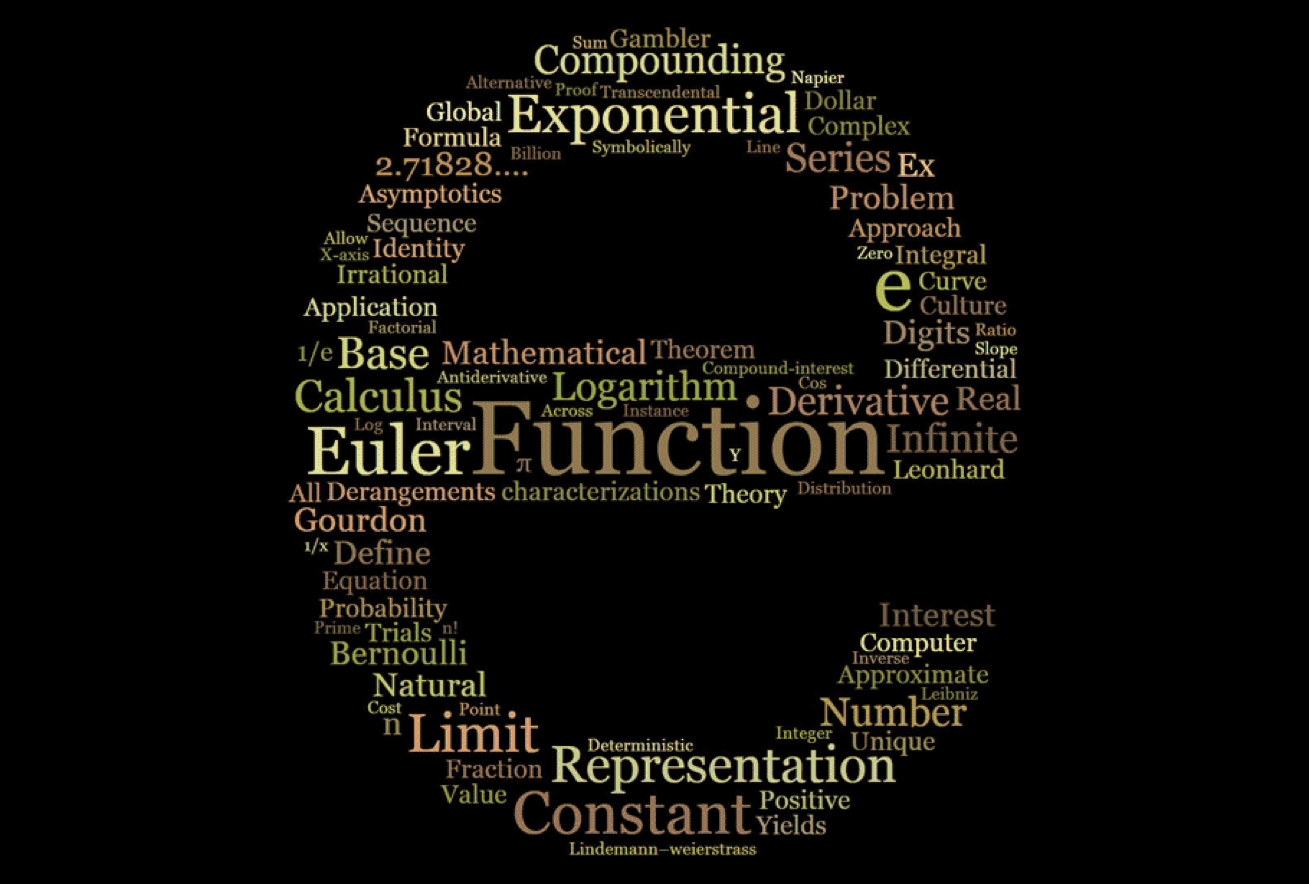
\includegraphics[scale=0.5]{google/eword.png}
\caption{$e$ 单词云}
\centering
\end{figure}


